\chapter{Results}\label{ch:re}
% These are the results I found from my investigation.

% Present your results in a suitable format using tables and graphs where necessary. Remember to refer
% to them in text and caption them properly.


% \section{Simulation Results}


% \section{Experimental Results}

All raw data can be found on \href{https://github.com/Neo-Vorsatz-UCT/eee4022s/blob/main/data/}{GitHub}.

\section{Latency}
The latency of the system due to each stage of the pipeline is shown in \autoref{fig_re:latency_boxplot} as a box and whisker plot. The mean and standard deviation of these latencies, as well as the total are shown in \autoref{tab_re:latency_table}.\\
The step response of the Braccio, approximated to 10\degree\space steps is shown in \autoref{fig_re:braccio_step}, along with a spline fit using $\lambda=2$ to help visualise the step.

\begin{figure}[h!]
    \centering
    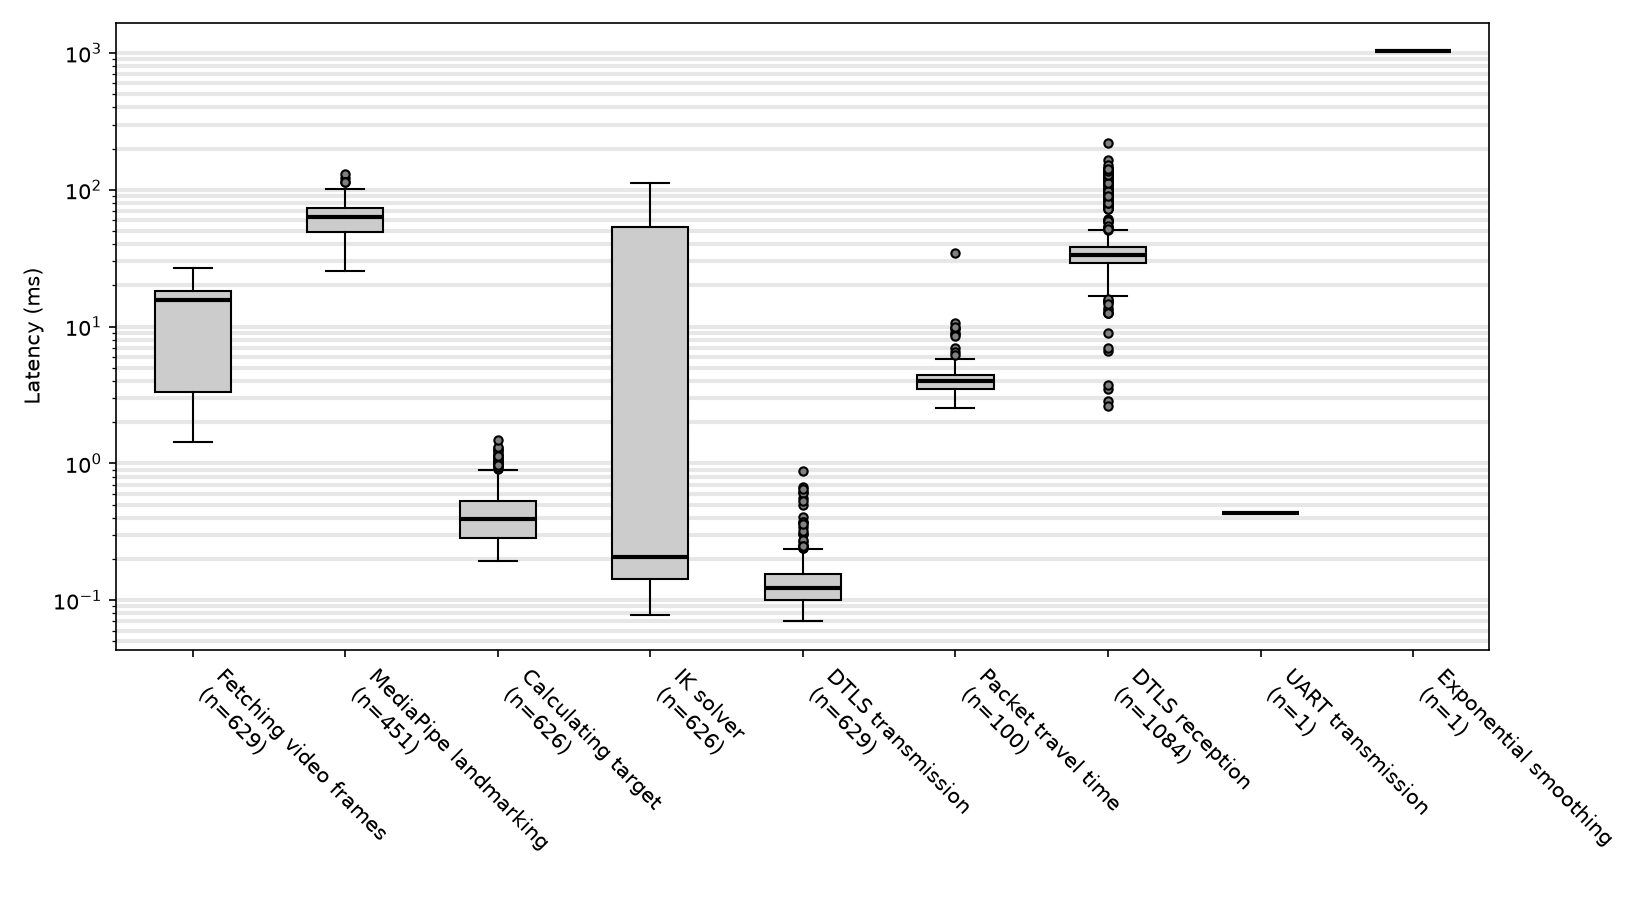
\includegraphics[width=1\textwidth]{graphics/results/latency_boxplot.png}
    \caption{Box and Whisker plot of latency contributed by each stage}
    \label{fig_re:latency_boxplot}
\end{figure}

\newpage
\begin{table}[h!]
\centering
\caption{Table of latency contributed by each stage}
\label{tab_re:latency_table}
\small{
\begin{tabular}{|l|c|c|c|c|}
    \hline
    \textbf{Stage} & \textbf{Mean (ms)} & \textbf{Standard Dev. (ms)} & \textbf{Number of Samples} & \textbf{Percentage of Total} \\
    \hline \hline
    Fetching video frames & 12.3 & 7.47 & 629 & 1.05\% \\
    \hline
    MediaPipe landmarking & 61 & 18.7 & 451 & 5.21\% \\
    \hline
    Calculating target & 0.438 & 0.199 & 626 & 0.0375\% \\
    \hline
    IK solver & 16.9 & 28.2 & 626 & 1.45\% \\
    \hline
    DTLS transmission & 0.139 & 0.0724 & 629 & 0.0119\% \\
    \hline
    Packet travel time & 4.7 & 3.42 & 100 & 0.402\% \\
    \hline
    DTLS reception & 40.4 & 24.4 & 1084 & 3.45\% \\
    \hline
    UART transmission & 0.438 & N/A & N/A & 0.0374\% \\
    \hline
    Exponential smoothing & 1,030 & N/A & N/A & 88.3\% \\
    \hline
    \hline
    \textbf{Total} & 1,170 & 42.5 & N/A & 100\% \\
    \hline
\end{tabular}
}
\end{table}

\begin{figure}[h!]
    \centering
    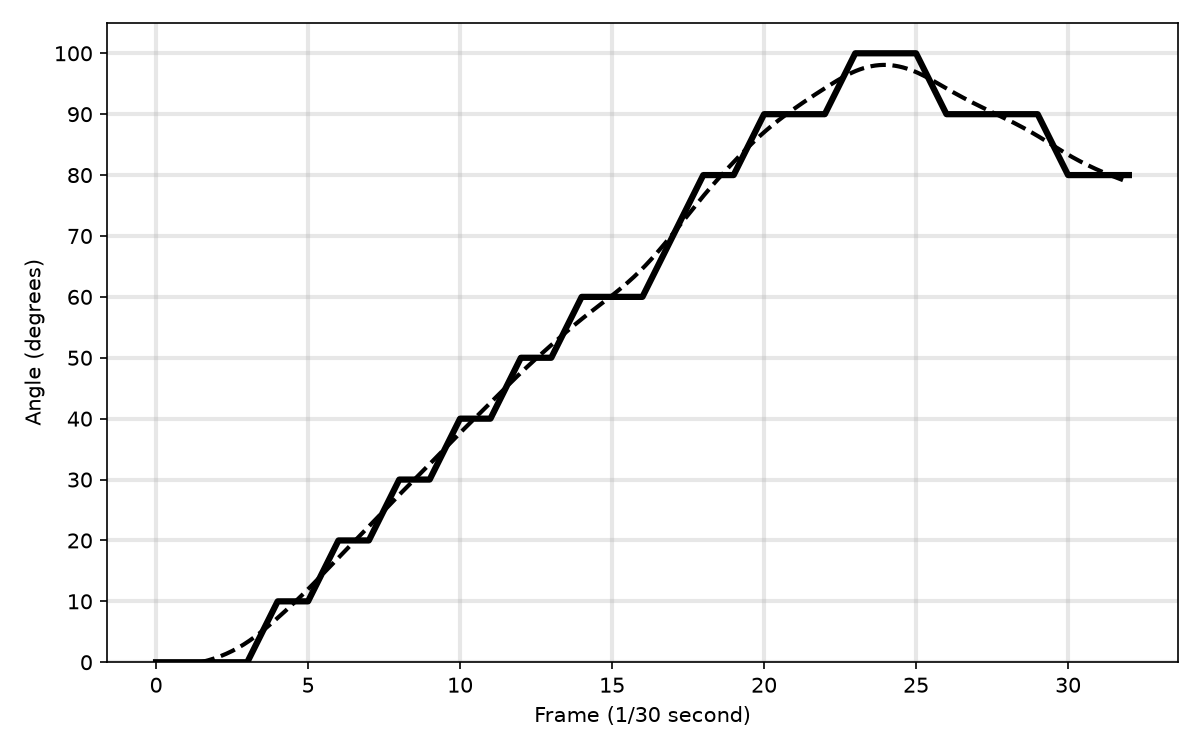
\includegraphics[width=1\textwidth]{graphics/results/actuation_line.png}
    \caption{Braccio arm step response}
    \label{fig_re:braccio_step}
\end{figure}

\section{Inverse Kinematics Solver}
The remaining error over time, after running the inverse kinematics solver, is shown in \autoref{fig_re:sqr_err}, while the latency and error per number of iterations is shown in \autoref{fig_re:lat_per_iter} and \autoref{fig_re:err_per_iter} respectively.

\newpage

\begin{figure}[h!]
    \centering
    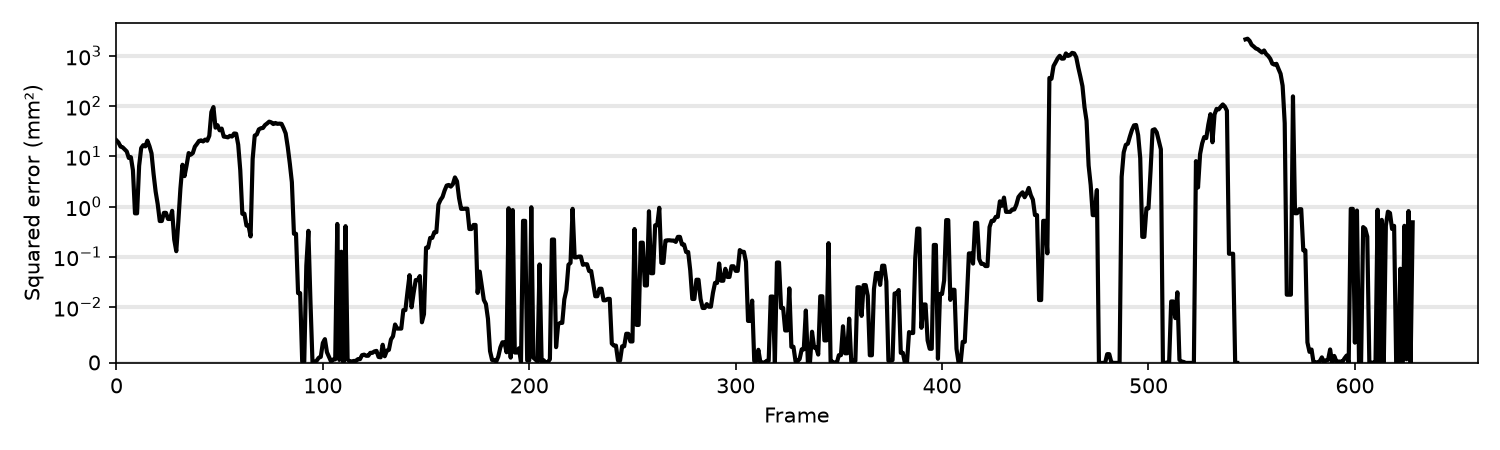
\includegraphics[width=\textwidth]{graphics/results/sqr_err.png}
    \caption{Squared error throughout the teleoperation task}
    \label{fig_re:sqr_err}
\end{figure}

\begin{figure}[h!]
    \centering
    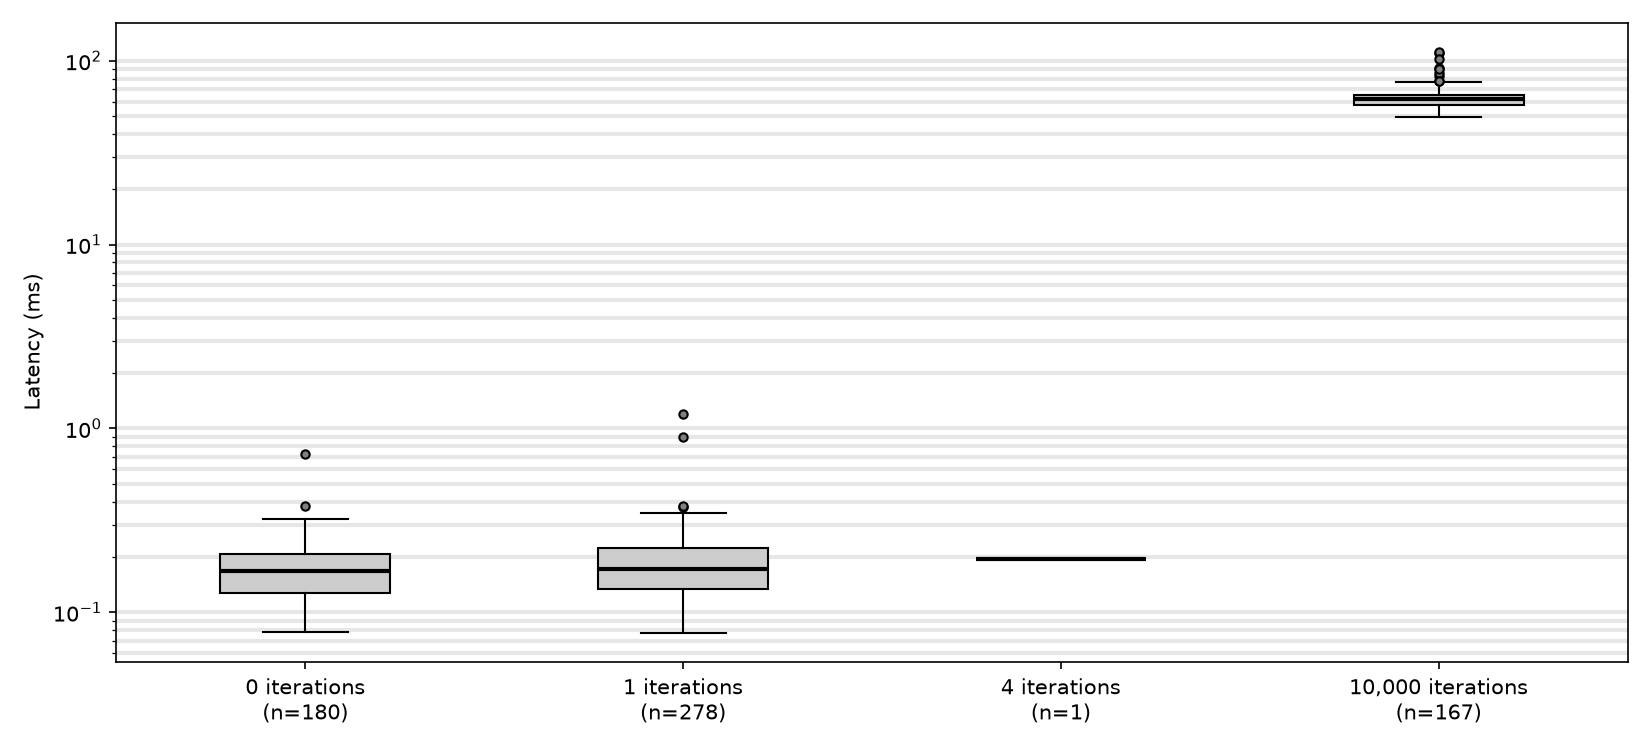
\includegraphics[width=\textwidth]{graphics/results/latency_per_iter.png}
    \caption{Latency per number of iterations}
    \label{fig_re:lat_per_iter}
\end{figure}

\begin{figure}[h!]
    \centering
    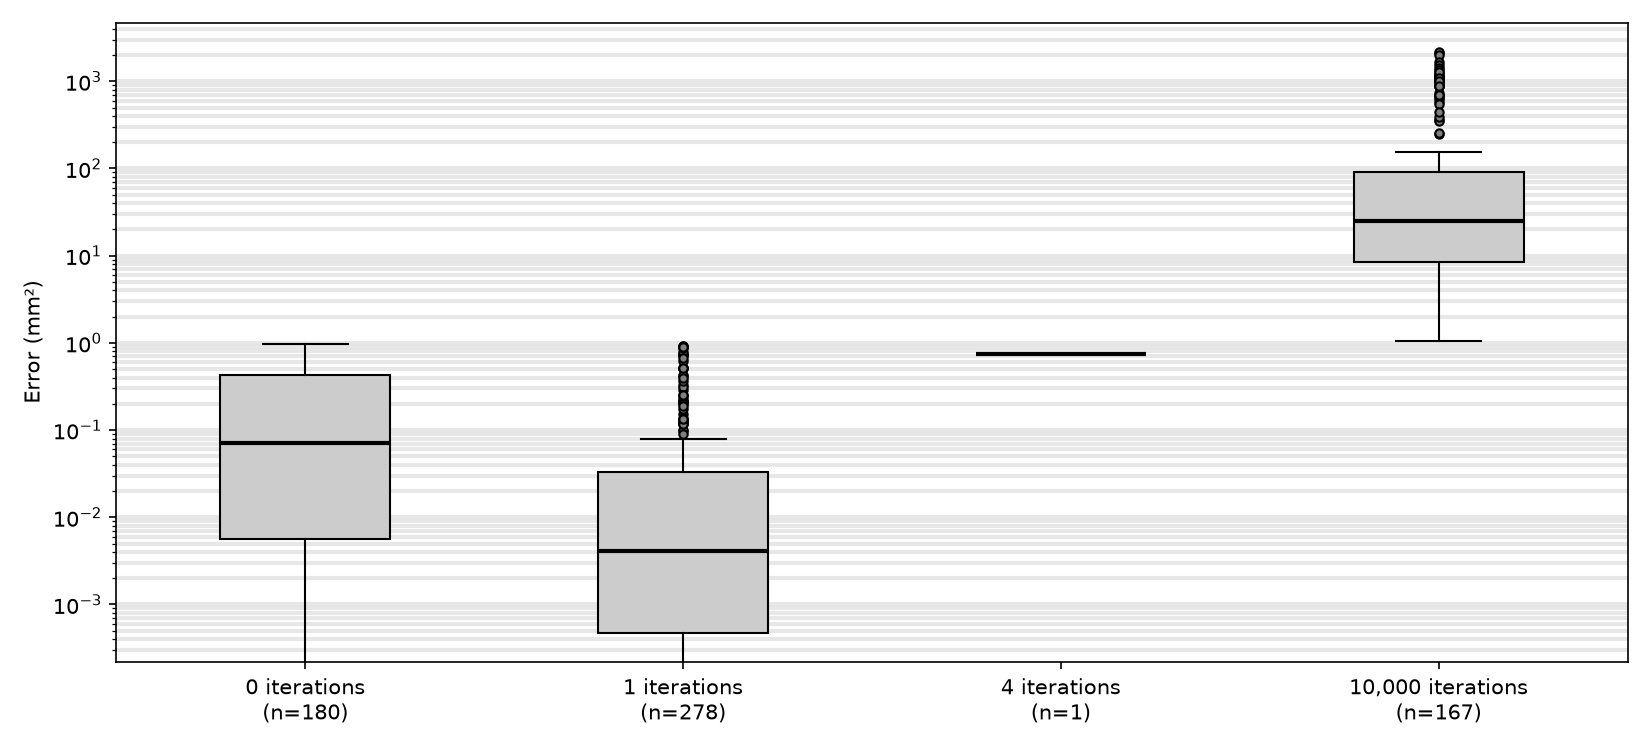
\includegraphics[width=\textwidth]{graphics/results/error_per_iter.png}
    \caption{Squared error per number of iterations}
    \label{fig_re:err_per_iter}
\end{figure}
